\begin{blocksection}
\question What would Python display? If an error occurs, write "Error". If a function is displayed, write "Function". If nothing is returned, write "Nothing".

\begin{lstlisting}
>>> a = [1, 2]
>>> a.append([3, 4])
>>> a
\end{lstlisting}
\begin{solution}[0.25in]
\begin{lstlisting}
[1, 2, [3, 4]]
\end{lstlisting}
\end{solution}
\end{blocksection}

\begin{lstlisting}
>>> b = list(a)
>>> a[0] = 5
>>> a[2][0] = 6
>>> b
\end{lstlisting}
\begin{solution}[0.25in]
\begin{lstlisting}
[1, 2, [6, 4]]
\end{lstlisting}
\end{solution}

\begin{lstlisting}
>>> a.extend([7])
>>> a += [8]
>>> a += 9
\end{lstlisting}
\begin{solution}[0.25in]
\begin{lstlisting}
TypeError: 'int' object is not iterable
\end{lstlisting}
\end{solution}

\begin{lstlisting}
>>> a
\end{lstlisting}
\begin{solution}[0.25in]
\begin{lstlisting}
[5, 2, [6, 4], 7, 8]
\end{lstlisting}
\end{solution}

Challenge:
\begin{lstlisting}
>>> b[2][1] = a[2:]
>>> a[2][1][0][0]
\end{lstlisting}
\begin{solution}[0.25in]
\begin{lstlisting}
6
\end{lstlisting}

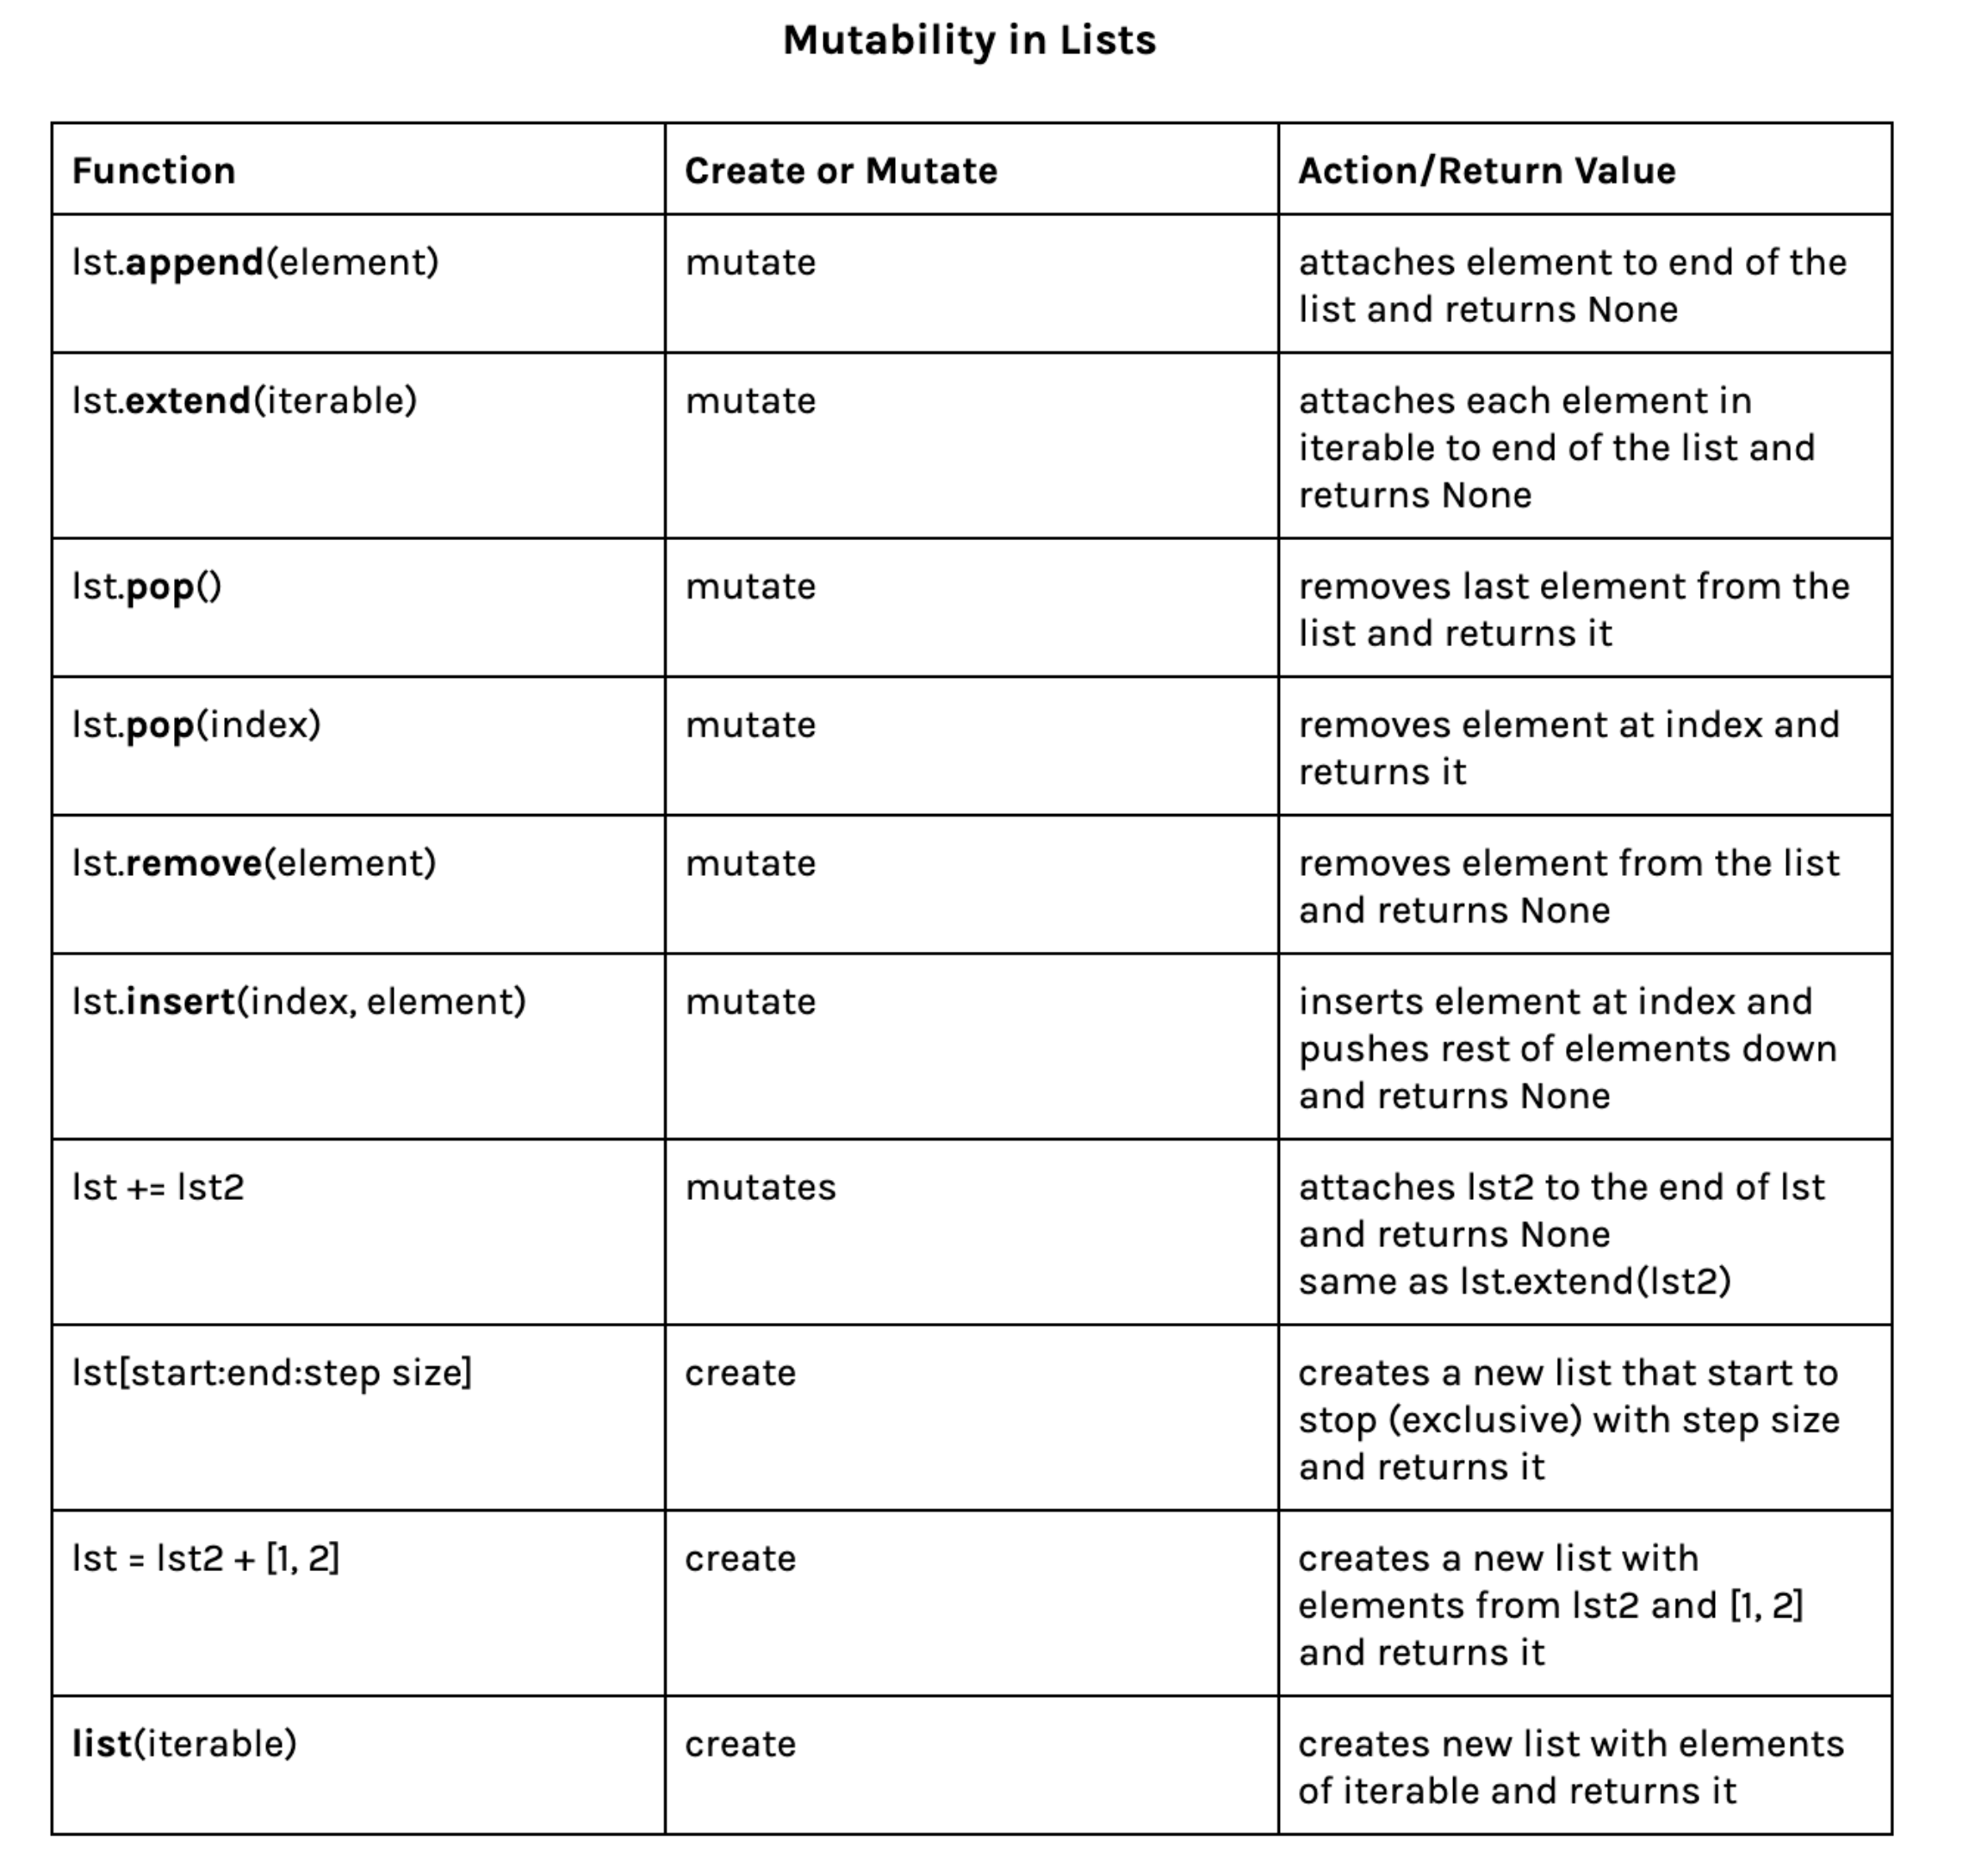
\includegraphics[width=.9\textwidth]{list-mutation.png}

\text{(credits: Mihira Patel)}
\end{solution}

\begin{blocksection}
	\begin{guide}
	\begin{itemize}
		\item Draw a box and pointer diagram
		\item Discuss shallow vs. deep copying. 
		\begin{itemize}
			\item Shallow copying is when you copy each element as is; i.e. elements which were pointers to a list still point to the same list in the copy.
			\item Deep copying is when you copy each element within each sublist; i.e. the new elements which are pointers point to brand-new created lists.
			\item In general, most operators involving Python lists perform shallow copying: i.e. slicing, list(...), etc.
		\end{itemize}
		\item If you have enough time, it is helpful for students to make a chart which the different operators and identify when to mutate or create a new list.
		\item Remind students of the difference between \lstinline{a += b} and \lstinline{a = a+b}. The former is essentially \lstinline{a.extend(b)}, while the latter creates a new list consisting of all the elements of \lstinline{a} and \lstinline{b} combined and binds it to \lstinline{a}.
	\end{itemize}
	\end{guide}
\end{blocksection}
	